\section{Introduction}

%LIGO is getting bigger and better, and running into new noise sources as the noise floor drops. Other detectors with an even better low frequency sensitivity will have a lot to worry about with angular controls.
%
%Angular traps are interesting to study because they have a number of potential uses in controlling the motion of optical components. They have the advantage of a much lower minimum noise than conventional sensing methods. They have the potential to   
%
%we demonstrate a trap for a 0.4 gram mirror in the position and yaw degrees of freedom.


%The Laser Interferometer Gravitational-wave Observatory (LIGO) is part of a world-wide  effort to detect gravitational waves and use them to study the universe \cite{BPAbbott09}. 
%Construction of LIGO's advanced detectors has finished and the first science runs have now begun. 
%We now look towards the next generation of gravitational-wave detectors, which will operate very close to the Standard Quantum Limit, meaning that the contributions from quantum radiation pressure and shot noise are about equal in the observation band \cite{Caves80, Ni86}.
%The goal of Advanced LIGO (aLIGO) is the first direct detection of gravitational-waves from astrophysical sources such as coalescing compact binaries and core-collapse supernovae.
%These detections will open a new spectrum for observing the universe and establish the field of gravitational-wave astronomy. 
%These initial observations will also show the potential science gain of further increasing the state-of-the-art sensitivity of gravitational wave detectors \cite{Smith09,Harry10,Losurdo12}.
%
%To design a successor to aLIGO, techniques to operate gravitational-wave interferometers below 
%the Standard Quantum Limit need to be developed \cite{Dan12, Chen13}. Dual carrier control systems and angular control 
%using stable optical springs are promising methods for evading quantum-mechanical limitations on 
%detector sensitivity \cite{LIGO10, Braginsky02b, Arcizet06b, Corbitt06b, Kippenberg05, Sheard04}. 
The Advanced LIGO detectors are now running and taking science data. Final upgrades should have the detectors at design sensitivity in a few years. At that point, we will need to have potential upgrades designed and demonstrated so that they can be considered for incorporation into the detectors.

One such area of interest is the use of radiation pressure to control of interferometer test masses.
The demonstration of radiation pressure control by Corbitt et al. showed that the method has a very strong promise \cite{Corbitt07}. 
%Although they did not completely turn off the low frequency feedback to the trapped mirror, 
%Their work clearly demonstrated the potential of this technique. 
%Extended to angular degrees of freedom, it has the prospect of opening a completely new approach to the angular control problem in future generation 
%gravitational-wave detectors \cite{Punturo10}. 
%Sidles and Sigg have shown that, for a Fabry-Perot cavity with a single resonating laser field, the radiation pressure force will couple the two end mirrors, always creating one soft (unstable) and one hard (stable) mode \cite{Sidles06}. 
We seek to extend radiation pressure control to two and possibly three degrees of freedom for use in gravitational wave detectors \cite{Punturo10}.

There is a significant radiation pressure effect called the Sidels-Sigg instability, which describes the coupling of two mirrors in a Fabry-Perot cavity via radiation pressure \cite{Sidles06}.
This sets a lower limit on the required angular control bandwidth. As laser power increases, this inevitably results in higher noise contamination by angular control noise.
 %and limits the angular control performance in the first and second generation gravitational-wave interferometers \cite{LIGO10, Braginsky01, Dooley13, Hirose10}. 
Angular optical trapping can damp the relative motion of test masses and control the Sidles-Sigg instability. 
Its fundamental noise limit is quantum radiation pressure noise, making it a promising candidate for low-noise angular control.


\section{Optical Springs}
In this chapter, we will discuss the control of a mirror using two pairs of optical springs, creating two stable degrees of freedom in a single mirror. One pair will be a executed in a straight cavity and one will be in a folded cavity. In a previous paper, we have derived the behavior of a single optical spring in a straight cavity:

\begin{eqnarray}
\label{eq:KOSlong}
K_{OS} & {\approx} & P_0 t_1^2 \frac{8k}{c(1-r_1r_2)^3}\frac{ \frac{\delta}{\gamma}}{(1+\frac{\delta^2}{\gamma^2})} 
\frac{1}{1+\frac{\delta^2}{\gamma^2}-\frac{\Omega^2}{\gamma^2}+i2\frac{\Omega}{\gamma} }.
\end{eqnarray}

In section \ref{sec:foldedOS}, we demonstrate the optical spring behavior of a folded cavity optical spring.
\begin{eqnarray}
\label{eq:KOSfolded}
K_{OS} & {\approx} & P_0 t_1^2 \frac{32k}{c(1-(r_1r_2)^2)^3}\frac{ \frac{\delta}{\gamma}}{(1+\frac{\delta^2}{\gamma^2})} 
\frac{1}{1+\frac{\delta^2}{\gamma^2}-\frac{\Omega^2}{\gamma^2}+i2\frac{\Omega}{\gamma} }.
\end{eqnarray}

We note that the only differences between the two equations are a factor of four in the numerator and the change of $r_1r_2$ to $(r_1r_2)^2$ in the denominator.

Because these beams are exerting force on a single mirror, we expect some crosstalk between the straight optical spring pair and the folded optical spring pair. We have attempted to minimize this though our choice of spot locations on the mirror (see appendix \ref{ap:beamseparation}).


\section{Setup}
Our experiment (see fig. \ref{f:experimentLayout}) uses a 2 Watt 1064 nm Nd:YAG laser. The laser beam is split into a carrier beam and a subcarrier beam, then the subcarrier is frequency shifted by a tunable amount, described in more detail in section IV of our previous paper \cite{Kelley15}. The two beams are mode matched and spatially recombined (in opposite linear polarizations) in a Mach-Zehnder-style setup. The recombined beam is then split using an unpolarized beamsplitter into main and side beams. The main beam enters the straight cavity, while the side beam enters the folded cavity. Both polarizations of both beams are monitored in transmission and reflection.



\begin{table}[htb]
\centering
\begin{tabular}{|l|l|l|}
\hline
Parameter & Straight & Folded \\ \hline
$\lambda_0$ & 1064 nm & 1064 nm \\ \hline
Mirror1,3,4 RoC & 7.5 cm & 7.5 cm \\ \hline
Mirror2 RoC & 5.0 cm & 5.0 cm \\ \hline
$L_0$ & 10.0 cm & 20.0 cm \\ \hline
M1,3,4 Spot size  & 268 $\mu$m & 268 $\mu$m\\ \hline
M2 Spot size  & 155 $\mu$m & 155 $\mu$m\\ \hline
FSR      & 1.50 GHz & 0.75 GHz \\ \hline
Finesse & 7500 & 3750 \\ \hline
Cavity Pole & 98.6 kHz & 98.6 kHz\\ \hline
Cavity angle, $\theta$ & 0 deg & 11 deg\\ \hline
\end{tabular}
\caption[Angular trap optical parameters]{Optical setup for the angular trap. The straight and folded cavities have different parameters due to the difference in total length and number of mirrors.}
\label{tab:longAngParams}
\end{table}


\begin{figure}[p]
\begin{center}
\includegraphics[width=.9\textwidth]{figures/Angular/simplifiedLayout}
\end{center}
\caption[Angular trap experiment layout]{%
\label{f:experimentLayout}
Layout of the angular trap cavity experiment.
The light from the laser is split into the carrier and subcarrier paths with a polarizing beam splitter (PBS), with a ratio determined by the $\lambda/2$ plate.
The subcarrier path is frequency shifted by two AOMs under the control of the subcarrier servo then recombined with the carrier with another PBS. 
The co-aligned mode-matched beams are then split into main and side paths, which enter the trap cavity.
The main beam has a straight optical path and is read out in transmission by broadband photodiodes and in reflection by RFPD1.
The side beam has a folded optical path and is read out in transmission by broadband photodiodes and in reflection by RFPD2.
We can use the 35 MHz modulation from the EOM with the two RFPDs in a PDH scheme to read out the cavity
lengths or lock the cavities.
}
\end{figure}

\section{Results}

We stably locked the main beam and achieved many concurrent two-second locks on the side beam using a transmitted power offset lock.

%We could not manage to stably lock the side cavity.
We could not extend the locks of the side cavity for longer periods due to a technical complication that I will describe below. We do not think that this is a fundamental problem. 
In the following subsections, I describe a few challenges, resolutions, and options for the further pursuit of side locking.

\subsection{Angular loop bandwidth}

\begin{figure}[htp]
\vspace{5pt}
\begin{center}
\includegraphics[width=.8\textwidth]{figures/Angular/ANGblocks2}
\end{center}
\caption[Folded cavity block diagram]{%
\label{f:angblocks}
Control loop structure for side cavity. Transmitted power is fed into yaw control for the input coupler.}
\end{figure}

The expectation was that we could lock the angular cavity after we locked the main cavity by pushing on the yaw of the optics.
Based on a calculation of range for the small optic, we could change the cavity length by $\lambda/2$ or one FSR by rotating the small optic about 20 $\mu$ rad. 
%theta = lambda/2 / 2.75 mm
The difficulty came in the bandwidth required to lock the side cavity.

Pushing on the yaw of the large optic results in a cavity length change of 2.9 $\mu m/m rad$, which means one FSR is about 190 $\mu rad$. 
This is due to the fact that you only change the length by the difference in the distance between the two side mirrors and the center of mass in the input coupler. 
%dL/dtheta = 2.87mm/rad
This means that we have a factor of 10 lower gain in feedback to the large mirror yaw, compared to that of the small mirror yaw.

Both optics have a yaw resonance around 1 Hz. The small mirror also has a yaw resonance around 22 Hz.
The more troubling thing is that something rings up in yaw around 66 Hz when we lock the side cavity. We are running out of range and the cavity loses lock. See figs \ref{f:sidelock} and \ref{f:sidelockspec}.

We think that the 66 Hz oscillation is a yaw mode of the ring suspension but it does not show up in the OSEMs. There are hints of the oscillation in the yaw optical lever signal after the resonance is rung up, so we should be able to clean up that signal and might be able to use that for damping feedback. 

\begin{figure}[htp]
\begin{center}
\includegraphics[width=\textwidth]{figures/Angular/sideLock.png}
\end{center}
\caption[Side Cavity lock attempt]{%
\label{f:sidelock}
Using a transmission power offset lock, we were able to temporarily achieve a concurrent lock of the main and side cavities. However, a yaw resonance in the small mirror suspension at about 66 Hz consistently rang up. Without enough control loop bandwidth, we could not damp this motion.}
\end{figure}

\begin{figure}[htp]
\begin{center}
\includegraphics[width=\textwidth]{figures/Angular/sideLockSpec.png}
\end{center}
\caption[Side Cavity lock spectrum]{%
\label{f:sidelockspec}
Spectrum of the two second lock shown in fig \ref{f:sidelock}. The four traces for show spectra taken every 0.5 seconds from $t=0$ to $t = 2.0$ The line at 66 Hz rings up over time. In the last trace, we can see the harmonics of 66 Hz also rung up.}
\end{figure}

\subsection{Resolving bandwidth issues}
\label{sec:bandwidth}

The biggest concern is to increase the bandwidth of the feedback system, so that we can damp this and other high-frequency modes. There are several approaches that could work. They are given in order of increasing invasiveness.

\subsubsection{Optical spring behavior}

By design, the small mirror is very strongly affected by radiation pressure. We could use this to our advantage, creating a stable optical spring to damp the motion. Otherwise, we could turn down the laser power or further detune it to reduce the energy coupling into the 66 Hz mode.


%If the resonance we see is due to optical spring effects, we should be able to flip the sign of the feedback to get damping.
%We could also drop the power or change the detuning.


\subsubsection{Improve OSEM diagonalization}
By improving the diagonalization in the two suspensions, we can reduce the amount of the dynamic range devoted to stabilizing the optics with respect to the suspensions and also possibly reduce the required bandwidth for the main cavity lock. This would free up more dynamic range for the side cavity lock.

\subsubsection{Inter-cavity coupling}
We saw a fair amount of power couple from the main cavity into the side cavity. This is probably caused by clipping or another source of scatter. This was temporarily fixed by changing the polarization of the side beam relative to that of the main beam, but this is not a good long-term solution, because the introduction of the carrier beam into the cavity will presumably cause carrier-to-subcarrier coupling for separate beams with the same polarization.

\subsubsection{Install AOM}
An AOM in a double-pass configuration could be used to actuate on one of the two paths, essentially introducing a variable frequency drive. 
We can get up to $\pm30$ MHz of actuation using a double-passed AOM, which should be plenty to cover the cavity pole (about 100 kHz). The significant challenge would lie in the behavior of the two different polarizations (carrier and subcarrier) in the AOM, which could lead to unacceptable losses.
This could be used for higher frequency feedback.

\subsubsection{Additional laser}
Setting up an entirely separate path would be the best way to guarantee that the side cavity could be locked, but it would require a lot of time and funds.

%\subsection{Angular interference}
%
%In the earlier stages of the experiment, we worried that the photothermal effect seen in the previous chapter could have a more significant impact due to interference patters on the mirror in the folded cavity. Using finite element modeling, we showed that this will not be an issue, because the heat will dissipate along the surface faster than heat can build up.
%
%\begin{figure}[htp]%
%\begin{center}
%\includegraphics[width=.8\textwidth]{figures/Angular/11deginterference}%lab\lab2014\OpticalLayout\20140903_angular_options
%\caption[Folded cavity interference pattern]{Simulated folded cavity interference pattern on the surface of M2. This corresponds to the power deposited into the mirror and thus the amplitude of the photothermal effect. Using this and the diffusion length as a function of frequency, we showed that there would be no significant amplification of the photothermal effect due to this distribution of absorbed power.}%
%\end{center}
%\label{fig:foldedinterference}%
%\end{figure}

\section{Noise sources}

There are four main players in this game:  The laser beam, the suspensions, the small mirror, and the seismic noise that couples into the system. 
The interactions between these components result in the vast majority of the noise that we expect to see in the output.

\subsection{Quantum Noise}

Quantum noise is unavoidable (though reducible via squeezing) in optical experiments.  The radiation pressure 
force $F_{RP}$ on the small mirror due to a laser with power $P$ can be written $F_{RP} = 2P/c$.  Quantum fluctuations $\Delta P$ in that power
cause a fluctuating force on the mirror which results in unwanted motion of that mirror. Thus we see that

\begin{eqnarray}
\Delta x = \frac{2 \Delta P}{{m c \left(-\omega^2+\omega_0^2+\frac{i\omega\omega_0}{Q}\right)}}.
\label{eq:dx/dP}
\end{eqnarray}


Two different things can affect the fluctuation in power.  Fundamentally, the shot noise in the system causes fluctuation.  Practically, the laser has some intensity noise that we can filter (using for instance the ISS), but we are nonetheless subject to.  The product manual says that the intensity noise should be less than $0.1\%$ of the RMS power between 10 Hz and 2 MHz.  With the ``noiseater'' option, we should be getting about -150 dB/$\sqrt{\mbox{Hz}}$ RIN (relative intensity noise).  This is about the same level as the shot noise.  The shot noise inside the cavity is given by

\begin{eqnarray}
\Delta P_{sn} = G\sqrt{\frac{2 h c P_{in}}{\lambda }}
\label{eq:sn}
\end{eqnarray}
where $P_{in}$ is the power entering the cavity, and G is the gain factor determined by the transmission and reflection coefficients of the two cavity mirrors.

\begin{eqnarray}
\sqrt{G} = t_1 e^{\frac{\imath \omega L}{c}} + t_1 r_1 r_2 e^{3\frac{\imath \omega L}{c}} \ldots = \frac{t_1 e^{\frac{\imath \omega L}{c}}}{1-r_1 r_2 e^{2\frac{\imath \omega L}{c}}}.
\label{eq:G}
\end{eqnarray}

We combine the shot noise for the positively and negatively detuned beams to get the total.

The motion caused by radiation pressure noise is also damped by the optical spring, so we multiply our answer by the closed-loop gain of the
spring-pendulum system.

%\begin{eqnarray}
%\frac{x}{F_{ext}} = \frac{1}{-m \omega^2+K_{tot}}
%\label{eq:TFkopt}
%\end{eqnarray}

Shot noise itself also plays a role in our measurement.  Our most accurate measurement of the small mirror motion is the PDH signal from the beam reflected by the cavity (because the sidebands are far from the cavity resonance).  By sweeping the mirror position, knowing the free spectral range (FSR) of our cavity, we can calibrate the PDH error signal to give us the change in the length of the cavity over time.

This measurement is limited by the quantum efficiency of the photodiode and the shot noise of the incoming light.  This shot noise is a function of the reflected power from the cavity.

It is important to note that this noise should not change the system, only hinder our ability to measure the system (unless we decide to feed back on the PDH signal).

%\begin{eqnarray}
%P_{ref} = P_{in}\left[\frac{r_1-r_2e^{2\imath \frac{\omega L}{c}}}{1-r_1r_2e^{2\imath \frac{\omega L}{c}}}\right]^2
%\label{eq:refPower}
%\end{eqnarray}

\begin{eqnarray}
P_{ref} = P_{in} \left[r_1 - \frac{t_1^2 r_2 e^{2\imath \frac{\omega L}{c}}}{1-r_1 r_2 e^{2\imath \frac{\omega L}{c}}} \right]^2.
\label{eq:refPower}
\end{eqnarray}

%The above equation is adapted from Haus (3.45).  We must make sure to apply it to both the carrier and subcarrier beams.
The above is the power reflected from a cavity.  Calculating this value for the carrier and subcarrier beams gives us the total reflected power.  
%
%From the carrier and subcarrier, we can obtain a total optical power reflected from the cavity, and thus the shot noise.
%
%The next question is how much of the power that gets to the photodiode is selected out by the mixer and the 25 MHz oscillator.

%\begin{eqnarray}
%P_{ref}+\Delta P = P_{in}\frac{r_1-r_2e^{2\imath \frac{\omega (L+\Delta L)}{c}}}{1-r_1r_2e^{2\imath \frac{\omega L}{c}}}
%\label{eq:refPowerDelta}
%\end{eqnarray}

%
%
%In this case, $\omega$ is the frequency of the detuned beam (we need to account for both the carrier and subcarrier).  Using the assumption that the displacement noise is very small, we can solve this for $\Delta L$
%
%\begin{eqnarray}
%e^{2\imath \omega (L+\Delta L)} \rightarrow e^{\frac{2 \imath}{c} \omega L} (1+\frac{2\imath}{c} \omega \Delta L) \equiv \phi A
%\label{eq:phi}
%\end{eqnarray}
%
%\begin{eqnarray}
%\Delta L = \frac{c}{2\imath \omega}\frac{\sqrt{P_{ref}+\Delta P}(1-r_1r_2\phi)\pm\sqrt{P_{in}}(r_1+r_2 \phi)}{\pm r_2 \phi \sqrt{P{in}}+r_1r_2\phi\sqrt{P_{ref}+\Delta P}}
%\label{eq:sndL}
%\end{eqnarray}

The shot noise is given by \cite{black} 

\begin{eqnarray}
S_P = \sqrt{\frac{2 h c P_{ref}}{\lambda}}.
\label{eq:Rsn}
\end{eqnarray}

We can express this as position noise of a Fabry-Perot cavity due to shot noise using the calibration of power to length in the reflected beam.

\begin{eqnarray}
S_L = \frac{\sqrt{h c}}{8} \frac{\sqrt{\lambda}}{F\sqrt{P_c}}.
\label{eq:SL}
\end{eqnarray}

In this equation, $P_c$ is the power in the carrier field; using the reflected power is a reasonable approximation.  $F$ is the cavity finesse. The calculated shot noise is several orders of magnitude below the dominant noise sources, so we shouldn't have to worry about it too much.  This effect could be increased if the carrier field of the beam was lower.

 
%when we drive an EOM in the path with a signal that looks like $V = V_0 \mbox{cos}(\omega_s t)$, it adds modulation to a beam: 
%
%\begin{eqnarray}
%E = e^{\imath\omega t+ \imath k d\frac{\partial n}{\partial V} V}\\
%E = e^{\imath\omega t+ \imath \Gamma \mbox{cos}(\omega_s t)}\\
%E = e^{\imath\omega t} e^{\left(\frac{\imath \Gamma}{2} \left[e^{\imath \omega_s t} + e^{-\imath \omega_s t}\right]\right)}\\
%E \approx e^{\imath\omega t} \left( 1+ \frac{\imath \Gamma}{2} \left[e^{\imath \omega_s t} + e^{-\imath \omega_s t}\right]\right)
%\label{eq:blah}
%\end{eqnarray}
%%
%  PUT STUFF HERE
%

We see a position noise due to the fundamental limits on our measurement.
Referred shot noise should just be inverse filtered by the cavity pole (but we do not see it because our cavity pole is much higher than our experiment bandwidth).

\subsection{Frequency Noise}

Fundamentally, the optical spring sees small fluctuations in laser frequency and small fluctuations in the cavity length as the same thing: a change in the detuning of the laser from the cavity resonance.  This means that laser frequency noise can be a significant contributor to the 'motion' seen by the spring, but it also means that the optical spring will move the cavity length to counteract changes in the laser frequency.

We know the frequency noise of the laser from the datasheet \footnote{Coherent,  \textit{Mephisto} coherent.com/downloads/Mephisto\_DS\_1013revA\_2.pdf}.  We can convert frequency noise to a position noise because we know the free spectral range (FSR) of the cavity and the wavelength; changing the frequency by one FSR is equivalent to moving the end mirror one wavelength.  We have to consider the round trip path for the laser, which introduces the factor of 2 in the denominator.

\begin{eqnarray}
x_fn = \delta f \frac{\lambda}{2 FSR}.
\label{eq:deltaf}
\end{eqnarray}

This is the apparent motion that would be introduced into an undamped cavity.  Because this cavity can react to the change in frequency, the effect is reduced by the closed loop gain of the optical spring system.

\subsection{Thermal Noise}
Thermal noise is broken up into two subsections: mirror and suspension.

For a suspension, we have to consider the dissipative/damping parts (because anywhere energy gets out, it can also get in!).

We'll be using a version of the Fluctuation-Dissipation Theorem:

\begin{eqnarray}
x_{therm}^2(f)=\frac{4 k_B T}{\omega^2} \mathfrak{R}(Z^{-1}(f)).
\label{eq:FDT}
\end{eqnarray}
Where $\mathfrak{R}(Z^{-1}(f))$ is the real part of the inverse of the impedance $Z$ of the system.  It is defined by the relation $F_{ext}=Z(f)v(f)$.  In other words, it's a measure of the force required to give your system a velocity $v$.  Thus we find

\begin{eqnarray}
\left(\frac{i \omega x}{F}\right)^{-1} \equiv Z=b+i \omega m -\frac{i k}{\omega} \\Z^{-1} = \frac{b+i(k/\omega-m\omega)}{b^2+(m\omega-k/\omega)^2	}. %= m\left(\frac{\omega_0}{Q} +i \omega  -\frac{i \omega_0^2}{\omega}\right)
\label{eq:Z}
\end{eqnarray}

At this point I should point out that we need to be careful about the difference between $k$, the effective spring constant of the small mass suspension, and $k_B$, Boltzmann's constant.  Combining Eqns. (\ref{eq:FDT}) and (\ref{eq:Z}) gives us an equation for the suspension thermal noise.  We're using the values for the position mode of the small suspension: $f_0 = 14.1$ Hz and $Q \approx 200$.  This value for $Q$ may be too low (which could lead to a lower-than-predicted thermal suspension noise). 

\begin{eqnarray}
x_{therm} = \frac{F_{therm}}{-m\omega^2} = \sqrt{\frac{4 k_B T b}{\omega^2(b^2+(\omega m -k/\omega)^2)}}.
\label{eq:thermalposnoise}
\end{eqnarray}

The mirror noise (including the coating and internal modes) is harder to predict, because the specifications on the coating are not freely given by the manufacturer.  I use the parameters for coating materials from Stefan Ballmer's angular trap proposal document.  The dominant noise (determined using GWINC\footnote{awiki.ligo-wa.caltech.edu/aLIGO/GWINC}) in the frequency range of interest is the coating Brownian noise.  I have used the \texttt{getCoatBrownian} function from GWINC to plot it.


\subsection{Seismic noise}

To calculate the seismic noise, we have to start with a spectrum measured in lab.  After that, we apply the transfer functions of the suspensions and the closed loop gain of the OSEM loops to get a good idea of how much noise we'll see.  We are curious mostly about position and bounce modes of vibration.  The position obviously concerns the trap, but the bounce modes of the two suspensions are distinct and very close to a strong peak in the Syracuse University seismic spectrum.  Unchecked, the seismic noise peak drives up the bounce modes, making the cavity unlockable.  The bounce mode can also couple to position through the pitch mode.  We have reduced this bounce mode by building small blade springs and fitting them to the top of the suspension, giving vertical isolation above 7 Hz.  We have implemented a feedback loop in the digital system to control the 7 Hz resonance via the bounce-to-pitch coupling.

\subsection{OSEMs}

Optical sensing electromagnets (OSEMs) are used in our experiment to position the large mirror and the ring supporting the small mirror.  We have glued small magnets onto the back side of the large mass and the ring. We sense the position of these magnets using pairs of LEDs and photodiodes in a `shadow sensor' configuration.  We feed this signal through a control loop, then actuate on a coil surrounding the shadow sensor.  These devices are limited by the shot noise of the shadow sensor.  We can calculate the effect of this noise on the mirror by multiplying the sensing noise by the position loop closed loop transfer function and the glass fiber suspension transfer function.  This seems to be somewhat limiting right now.  It may be beneficial to change the loop.


\begin{figure}[htp]
\centering
\includegraphics[width=\textwidth]{figures/Angular/angNoise}
\caption[Angular trap noise prediction]{%
\label{f:angularNoise}
Expected noise budget for the angular trap. The noises associated with mirror position motion or frequency noise are damped by an expected optical spring. At low frequencies, the total noise is dominated by seismic noise. Starting around 10 Hz, we see the effects of OSEM noise and laser frequency noise dominating the noise spectrum. At very high frequencies, we see the effects of thermal noise at the resonant frequencies of the optical springs.
}
\end{figure}


\section{Folded cavity optical spring derivation}
\label{sec:foldedOS}
To determine the behavior of a folded optical spring, we can compare it to the standard optical spring derivation \cite{Perreca14}.

We begin with a folded cavity with three mirrors, shown in fig. \ref{f:angularLayout}. We assume that M3 and M4 have the same amplitude reflectivity as M1, $r_1$, while we allow the end mirror to have a different reflectivity, $r_2$. The incoming field is $E=e^{\frac{i 2 \pi c t}{\lambda}}$. The average round-trip path length is $L = 2L_0$, where $L_0$ is the optical patch length between mirrors M3 and M4. We consider microscopic changes in cavity length $d_n$, which are discreet samples of a harmonic oscillation $d(t) =  x_0 e^{i\Omega t}$. The light travel time between M3 and M4 is $\tau = \frac{L_0}{c}$. It is important to note that the cavity length $L_0$ of the folded cavity is twice that of the straight cavity in our experiment.

\begin{figure}[htp]
\vspace{5pt}
\begin{center}
\includegraphics[width=.5\textwidth]{figures/Angular/angularLayout}
\end{center}
\caption[Folded cavity layout]{%
\label{f:angularLayout}
Layout of the angular trap cavity. Light enters through mirrors M1 and M3. The angle $\theta$ of the folded cavity is measured from the normal of M1. 
}
\end{figure}

We can use the same $X$ and $Y$ notation as the original derivation in Chapter \ref{ch:theory} with one small change. $Y=e^{-i\Omega 2\tau}$ is the same, but now $X=(r_1r_2)^2 e^{\frac{-i2\pi L}{\lambda}}$ because the optical path touches M3 and M4 once and M2 twice.

We consider a set of displacements $d_n$, discretely sampled from a continuously oscillating function. This is equivalent to driving the cavity length at angular frequency $\Omega$.  
\begin{eqnarray}
d(t) = x_0e^{i \Omega(t-(2n-1)\tau)}\\
d_1 = x_0e^{i \Omega(t-\tau)}\\
d_n = Y^{2n-2}d_1  .
\end{eqnarray}

Following \cite{Perreca14}, we get an equation for the electric field in the cavity, which we must change to reflect that we can only have real values for $d_1$.

\begin{eqnarray}
\label{e:Etot}
E_{tot} = \frac{t_1 E}{1-X}\left[ 1- \frac{4i\pi d_1}{\lambda}\frac{X}{1-Y^2X}\right]\nonumber\\
E_{tot} = \frac{t_1 E}{1-X}\left[ 1- \frac{4i\pi}{2\lambda}\left(\frac{ d_1}{1-Y^2X}+\frac{ \overline{d}_1}{1-\overline{Y}^2X}\right)\right].
\end{eqnarray}

Then we get the cavity power:

\begin{eqnarray}
\label{e:P}
P&=&E_{tot}\cdot \overline{E}_{tot}=-P_0 t^2\left[ \frac{i 2\pi Y}{\lambda(1-X)(1-\overline{X})}\left(\frac{X}{1-Y^2X}-\frac{\overline{X}}{1-Y^2\overline{X}}\right)\delta L+cc\right] .
%&-&\frac{ikX xY}{(1-\overline{X})(1-X)(1-Y^2 X)} -
%\frac{ikX \bar{x}\overline{Y}}{(1-\overline{X})(1-X)(1-\overline{Y}^2 X)}\nonumber \\
%&+&\frac{ik\overline{X} \bar{x}\overline{Y} } {(1-\overline{X})(1-X)(1-\overline{Y}^2 \overline{X})}+ 
%\frac{ik\overline{X} xY}{(1-\overline{X})(1-X)(1-Y^2 \overline{X})}]  \nonumber \\
%P &=&-P_0t^2 \left[ \frac{ikY}{(1-\overline{X})(1-X)} \left( \frac{X(1+Y^2)}{1-Y^2 X}-\frac{\overline{X}(1+\overline{Y}^2)}{1-Y^2\overline{X}} \right) x + cc \right]?
\end{eqnarray}

We add an extra $Y^{1/2}$ term to get to the other side of the cavity.
It is important to note that the change in cavity length $\delta L$ used here is strictly that: the cavity length. If we want to transpose that into longitudinal change, we need to multiply by a geometric factor (see fig. \ref{f:angularLayout}):

\begin{equation}
\delta L = \frac{2 \delta z}{\mbox{cos}(\theta)}.
\label{e:deltaL}
\end{equation}

There is similarly a geometric correction when calculating the radiation pressure force $F_{rad}$

\begin{eqnarray}
F_{rad} &=& \frac{2r_2^2}{c} P (2 \mbox{cos}(\theta)) = -K_z \delta z\\
&=& \frac{2r_2^2}{c} (2 \mbox{cos}(\theta)) P_0 t^2\left[ \frac{i 4\pi Y^{3/2}}{\lambda(1-X)(1-\overline{X})}\left(\frac{X}{1-Y^2X}-\frac{\overline{X}}{1-Y^2\overline{X}}\right)\frac{2 \delta z}{\mbox{cos}(\theta)}+cc\right]. \nonumber
\label{e:Frad}
\end{eqnarray}

thus 
\begin{equation}
K_z=\frac{8r_2^2}{c} P_0 t^2 \frac{i 4\pi Y^{3/2}}{\lambda(1-X)(1-\overline{X})}\left(\frac{X}{1-Y^2X}-\frac{\overline{X}}{1-Y^2\overline{X}}\right).
\label{eq:Kz}
\end{equation}

With detuning:

\begin{equation}
X \rightarrow X=(r_1r_2)^2 e^{-i2\delta\tau}.
\label{e:Xdet}
\end{equation}
Here $\delta = \omega_0-\omega_{res}$, the angular frequency detuning from the cavity resonance, $\omega_{res} = 2\pi n c/L$, and $\omega_0$ is the frequency of the laser.

\begin{eqnarray}
K_{OS}=&-P_0 t^2 r_2^2 \frac{32i\pi e^{-\frac{3}{2}i\Omega\tau}}{\lambda c(1-(r_1r_2)^2e^{i2\delta\tau})(1-(r_1r_2)^2e^{-i2\delta\tau})}\times\nonumber\\
 & \left( \frac{(r_1r_2)^2e^{-i\delta \tau}}{1-(r_1r_2)^2e^{-2i\Omega\tau} e^{-i2\delta\tau}}
 -\frac{(r_1r_2)^2e^{i2\delta\tau}}{1-(r_1r_2)^2e^{-2i\Omega\tau}e^{i2\delta\tau}} \right). 
\end{eqnarray}

The finesse for the folded cavity is $F = \pi\frac{FSR}{\gamma} \approx \frac{\pi}{1-(r_1r_2)^2}$, which is half that for a straight cavity using the same mirrors. Since the FSR is also half of that for the straight cavity, $\gamma$ is the same here as it is for the longitudinal trap.

\begin{eqnarray}
\label{eq:KOSfold}
K_{OS} & {\approx} & P_0 t_1^2 \frac{32k}{c(1-(r_1r_2)^2)^3}\frac{ \frac{\delta}{\gamma}}{(1+\frac{\delta^2}{\gamma^2})} 
\frac{1}{1+\frac{\delta^2}{\gamma^2}-\frac{\Omega^2}{\gamma^2}+i2\frac{\Omega}{\gamma} }.
\end{eqnarray}

Comparing this result to the same result for a straight cavity (Eq. \ref{eq:KOSlong}), we see that the folded cavity spring constant is four times larger in magnitude than a similar straight cavity, and there is a change of $r_1r_2$ to $(r_1r_2)^2$.
